% 问题四
\section{问题四：任务分区与资源配置}
\label{sec:p4}

\subsection{问题分析}

问题四要求把 15 个服务区划分为两组与三组两种方案，按组配备运输无人机、电池、
中继无人机与能源组件，含冗余备份，并说明各组能否独立完成保障任务。问题四把分区与资源配置作为联合决策：分区应使各组的地理与通信需求自洽，即尽量让一组
对应一个中继布设点及其覆盖的服务区；资源配置应满足各组独立作业的时限与容量
要求，同时冗余备份需纳入库存核算。

\subsection{分区方案}

由第\ref{sec:p3}节的结论，三个中继布设点分别服务西与北片区、东片区
与 S004，且 S004 必须独立中继；第六节的 29 架次冠军全部为单区架次，
不存在跨区架次，故"同一架次涉及的服务区必须同组"的规则对分区不构成额外
约束。据此给出两种自然分区，图 \ref{fig:p4part} 以三组方案示意。

\begin{itemize}
\item 三组方案：G1 为西与北 10 区，即 S001、S002、S003、S005、S006、S007、
S008、S009、S011、S015，共 62 箱；G2 为东 4 区，即 S010、S012、
S013、S014，共 12 箱；G3 为 S004，共 6 箱。
\item 两组方案：G1 为西与北 10 区加 S004，共 11 区 68 箱；G2 为东
4 区。
\end{itemize}

\begin{figure}[htbp]
\centering
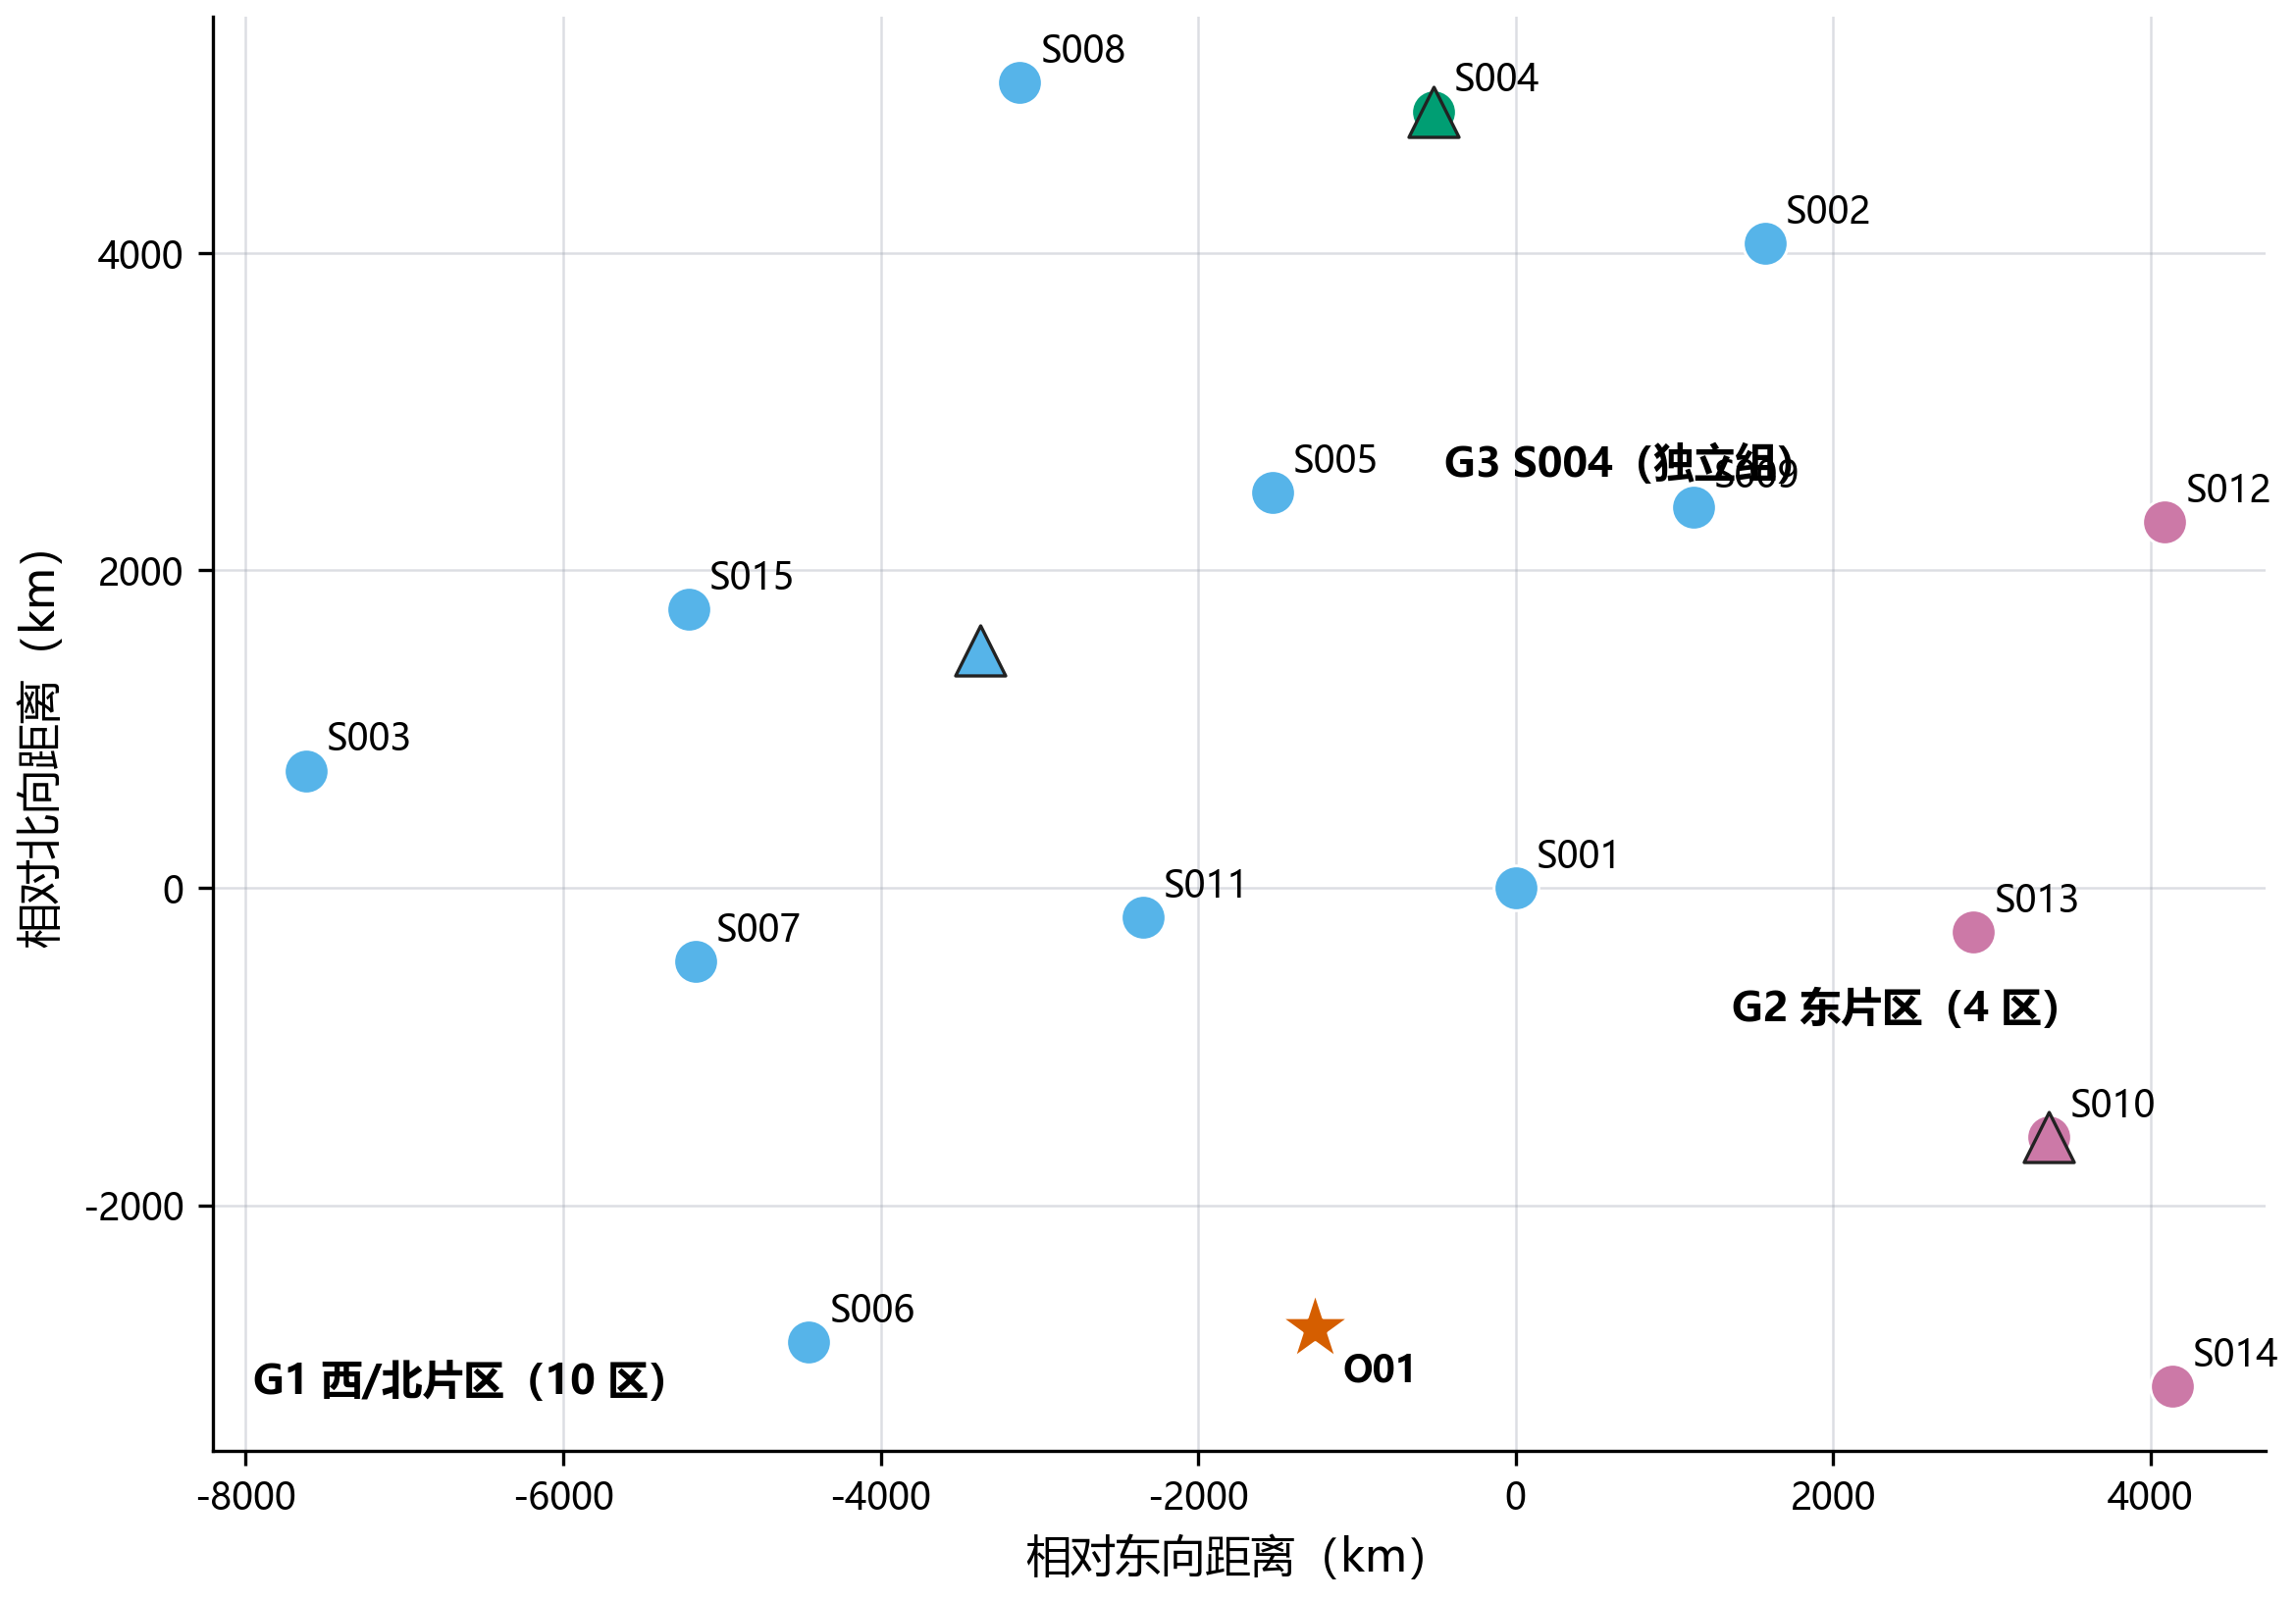
\includegraphics[width=0.76\textwidth]{figures/p4_partition.png}
\caption{三组任务分区示意（G1 西与北片区、G2 东片区、G3 为 S004）}
\label{fig:p4part}
\end{figure}

两种分区的各组负荷对比见图 \ref{fig:load}：三组方案把重载的西与北片区独立
为 G1，G2 轻载由 A/B 型自足，G3 的 S004 极小但须独享中继；两组方案把 S004
并入 G1，G1 负荷明显增大。

\begin{figure}[htbp]
\centering
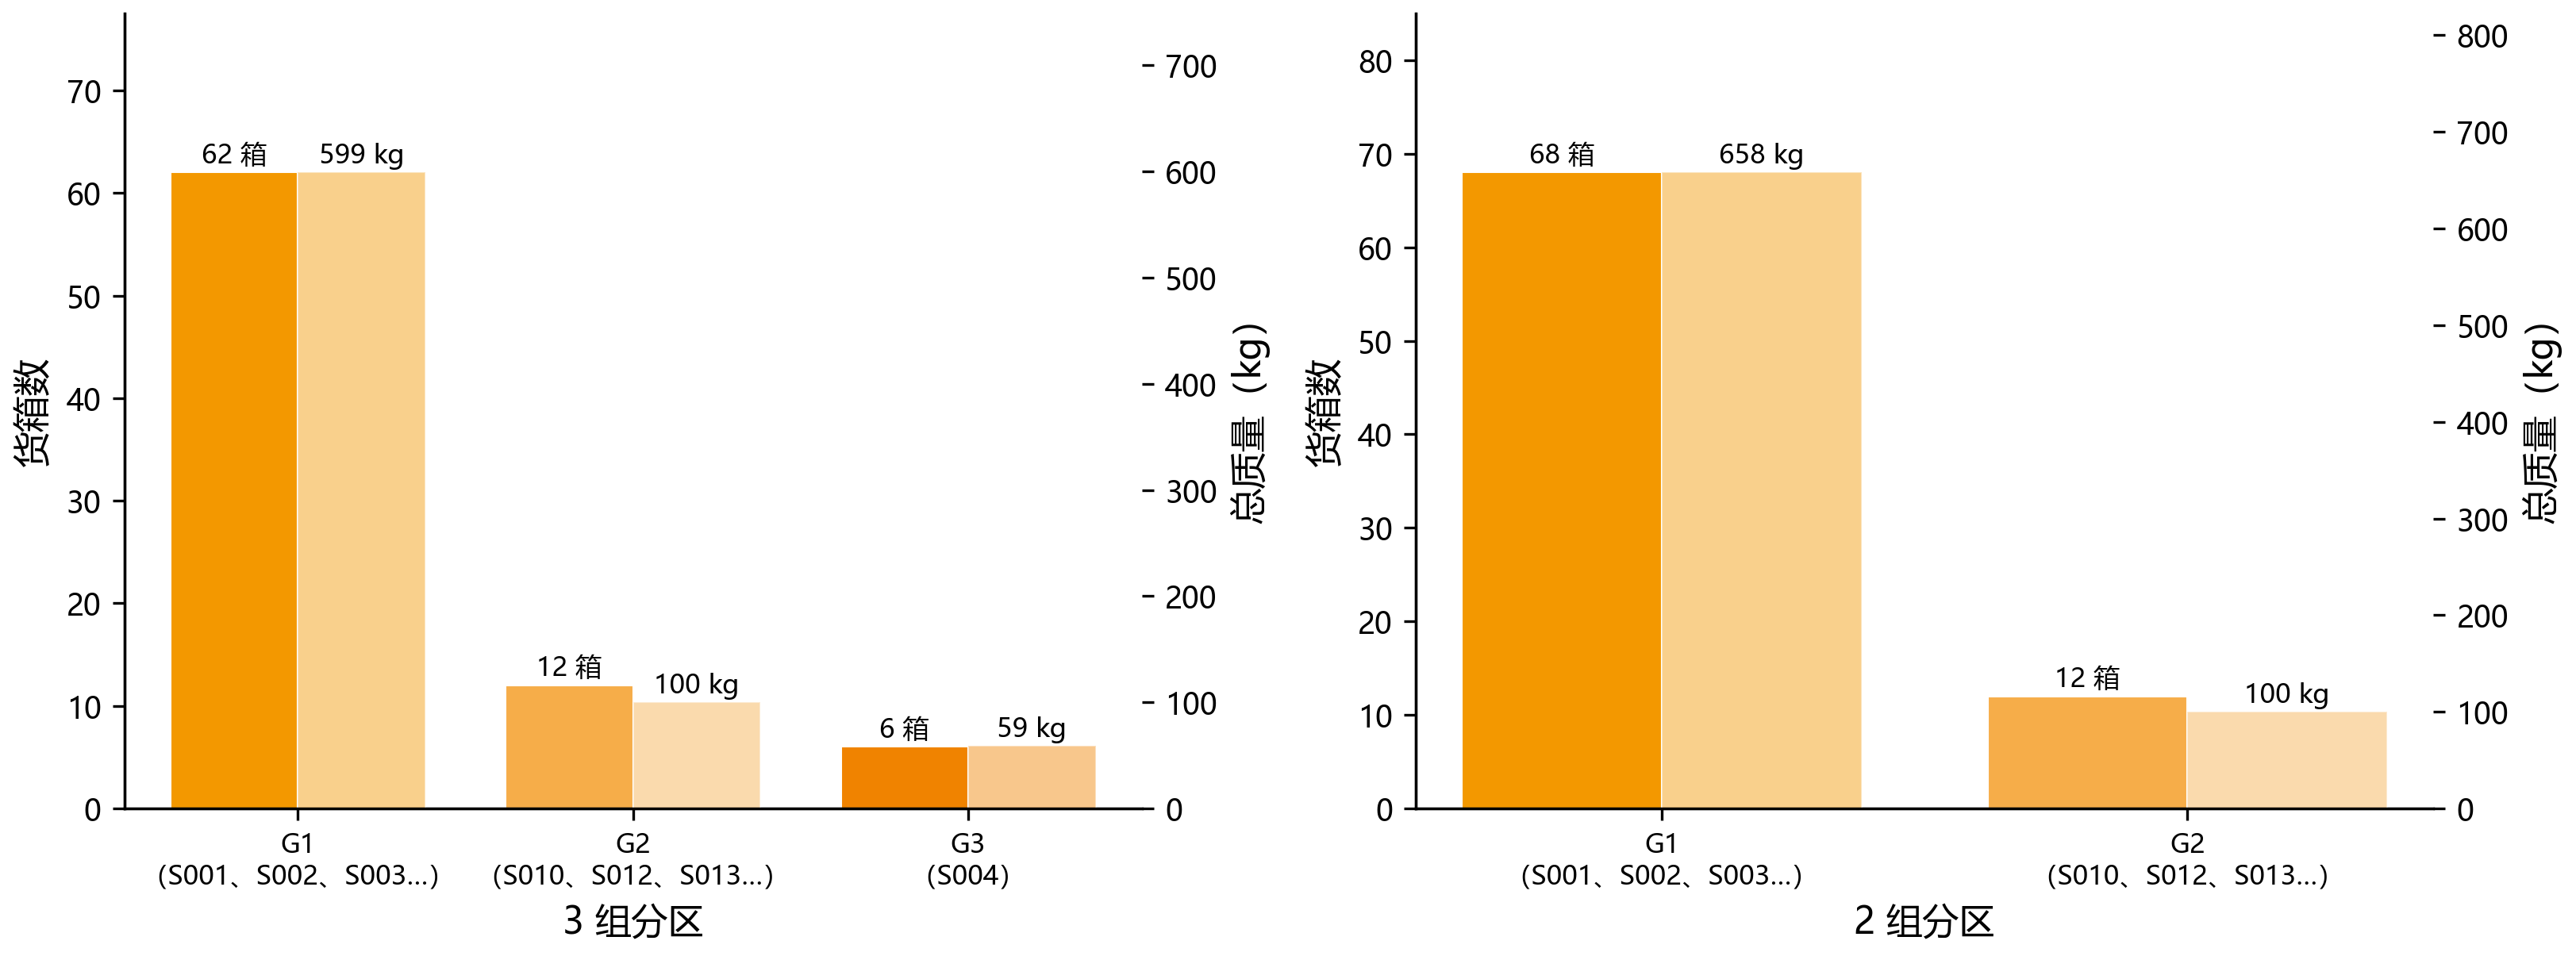
\includegraphics[width=0.98\textwidth]{figures/p4_load.png}
\caption{三组与两组方案各组货箱数与总质量对比}
\label{fig:load}
\end{figure}

\subsection{最小机队求解}

对每组执行最小机队搜索：把第六节协同方案中属于该组的货箱与架次拆出，以调度器
资源限额参数遍历机型组合与电池冗余数量，求满足全部硬时限且加权迟到为零的最小
机队。结果如表 \ref{tab:p4} 所示，各组均存在零迟到方案：三组方案下 G1（西与北
10 区）完工约 167\,min，G2（东 4 区）约 90\,min，G3（S004）约 36\,min；两组方案下
G1（西与北 10 区加 S004）完工约 155\,min，G2 约 90\,min。各组的在用机型与电池均
由 A、B、C 三类分担，其中 G1 需较多 A 型机轮转，G2 以 A/B 型自足，S004 只需
A/C 两类各 2 机。

\subsection{冗余备份与库存核算}

按在用机型加一架、电池加一组、中继加一架的方式计入冗余备份，得到各组配备
方案，见表 \ref{tab:p4}，完整明细见《结果提交模板》Q4 工作表。

\begin{table}[htbp]
\centering
\caption{分区资源配置方案（最小机队加冗余备份）}
\label{tab:p4}
\small
\begin{tabular}{llcccccccccc}
\toprule
K & 组 & 服务区 & A机 & B机 & C机 & A电 & B电 & C电 & 中继 & 组件 & 完工(s) \\
\midrule
3 & G1 & 西/北10区 & 3 & 2 & 3 & 5 & 4 & 5 & 2 & 11 & 10047 \\
3 & G2 & 东4区 & 2 & 2 & 0 & 3 & 3 & 0 & 2 & 4 & 5414 \\
3 & G3 & S004 & 2 & 0 & 2 & 2 & 0 & 2 & 3 & 2 & 2177 \\
\midrule
2 & G1 & 西/北10区+S004 & 4 & 2 & 3 & 6 & 4 & 5 & 3 & 10 & 9291 \\
2 & G2 & 东4区 & 2 & 2 & 0 & 3 & 3 & 0 & 2 & 4 & 5414 \\
\midrule
\multicolumn{3}{l}{库存} & 4 & 2 & 2 & 6 & 4 & 4 & 2 & 6 & --- \\
\bottomrule
\end{tabular}
\end{table}

\subsection{独立保障能力结论}

若坚持按组完全独立配置且含冗余，两种方案均超出给定库存。两组方案合计需
A 型机 6 架、B 型机 4 架、C 型机 3 架，分别超出库存 2、2、1 架；A 型电池 9 组、
B 型 7 组、C 型 5 组，分别超出 3、3、1 组；中继 5 架超出 3 架，能源组件 14 组
超出 8 组。三组方案分组更细导致重复配置更多，A 型机、B 型机、C 型机分别超出
3、2、3 架，A 型电池超出 4 组，中继超出 5 架，能源组件超出 11 组。缺口成因有三，
其一为西与北 G1 的 A 型任务集中，独立运转需 4 机与多组电池轮转，而轻载组也不能缺
机型保障；其二为 S004 的北点中继与各组自身中继需求并发，每组都要中继冗余；
其三为分组越细，重复配置越多，即三组方案缺口大于两组方案。

因此，在给定库存下更优的组织方式是任务分区与资源池化，即分区仅用于任务组织
与指挥协同，机队、电池与中继仍由调度中心集中调度并按时间分片复用。这正是
第六节协同方案的做法，以 8 架运输机、14 组电池、2 架中继分片服务三个时段，
恰好覆盖全部任务；零迟到与零盲区均在库存内实现。若必须完全独立按组
配置，则需增配 A 型机 2 至 3 架、B 型机 2 架、C 型机 1 至 3 架、A 型电池 3 至
4 组、B 型电池 3 组、中继 3 至 5 架与能源组件 8 至 11 组。两组与三组
方案的资源需求相对库存的缺口对比见图 \ref{fig:gap}，红色标注为超出库存的
数量，可见缺口集中在运输机与电池，且分组越细缺口越大；该结论的工程含义是：应急条件下中继等高价值资源应集中管理、按需调度；
分区用于组织指挥，不切割资源配置。

\begin{figure}[htbp]
\centering
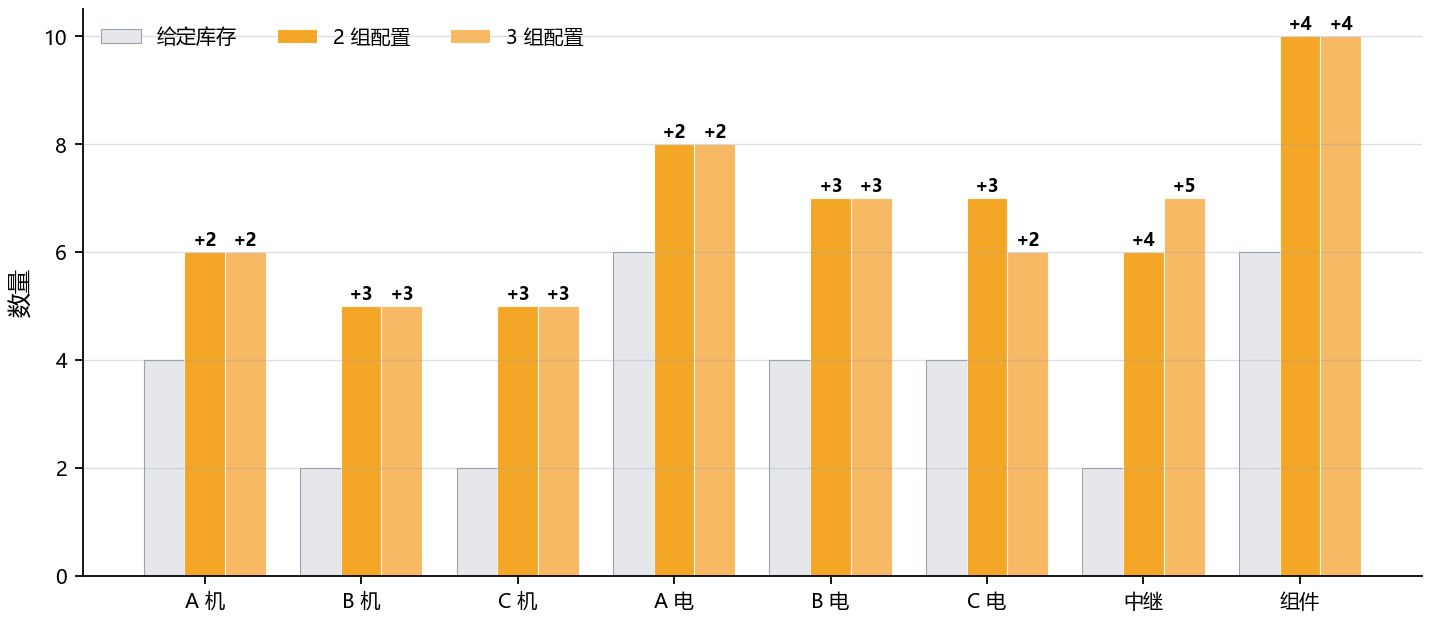
\includegraphics[width=0.96\textwidth]{figures/p4_gap.png}
\caption{两组与三组方案资源配置相对库存的缺口对比}
\label{fig:gap}
\end{figure}